% $Id: rfssample.tex,v 19:a118fd22993e 2013/05/24 04:57:55 stanton $
\documentclass[11pt]{article}

% DEFAULT PACKAGE SETUP
\usepackage{soul}
\usepackage{paralist}
    \newenvironment{paraenum}{\begin{inparaenum}[\itshape a)\upshape]}{\end{inparaenum}}
\usepackage{tabularx}
\usepackage{changepage,threeparttable}
\usepackage{tikz} 
\usepackage{pgf-pie} 
\usepackage{pgfplotstable}
\usepackage{pgfplots}
    \usepgfplotslibrary{groupplots,dateplot}
    \pgfplotsset{compat=newest}
    
  \newcommand{\globalTikzScale}{1}

  \newcommand{\axisHeight}{5cm}
  \newcommand{\axisWidth}{10cm}
  \newcommand{\barWidth}{0.25cm}
  
\definecolor{barFillColor1}{rgb}{1,1,1}
\definecolor{barDrawColor1}{rgb}{0,0,0}

% Bar charts which have only 2 plot
% Second colors
\definecolor{barFillColor2}{rgb}{0,0,0}
\definecolor{barDrawColor2}{rgb}{0,0,0}

% Bar charts which have only 1 plot
\definecolor{barFillColor}{rgb}{1,1,1}
\definecolor{barDrawColor}{rgb}{0,0,0}

% Pie Charts
\definecolor{pieFillColor}{rgb}{1,1,1}
\usepackage{setspace,graphicx,epstopdf,amsmath,amsfonts,amssymb,amsthm,versionPO}
\usepackage{marginnote,datetime,enumitem,subfigure,rotating,fancyvrb}
\usepackage{hyperref,float}
%\usepackage[sort&compress]{natbib}
%\usepackage[longnamesfirst]{natbib}
\usepackage[round,authoryear]{natbib}
%\setcitestyle{authoryear}
%\usepackage[capitalize, noabbrev]{cleveref}
\usepackage[capitalize]{cleveref}
\usdate

% Make subsubsections inline with a period after the title
\usepackage{titlesec}
\newcommand{\periodafter}[1]{#1.}
\titleformat{\subsubsection}[runin]
{\normalfont\bfseries}{\thesubsubsection}{1em}{\periodafter}

% These next lines allow including or excluding different versions of text
% using versionPO.sty

\excludeversion{notes}		% Include notes?
\includeversion{links}          % Turn hyperlinks on?

% Turn off hyperlinking if links is excluded
\iflinks{}{\hypersetup{draft=true}}

% Notes options
\ifnotes{%
\usepackage[margin=1in,paperwidth=10in,right=2.5in]{geometry}%
\usepackage[textwidth=1.4in,shadow,colorinlistoftodos]{todonotes}%
}{%
\usepackage[margin=1in]{geometry}%
\usepackage[disable]{todonotes}%
}

% Allow todonotes inside footnotes without blowing up LaTeX
% Next command works but now notes can overlap. Instead, we'll define 
% a special footnote note command that performs this redefinition.
%\renewcommand{\marginpar}{\marginnote}%

% Save original definition of \marginpar
\let\oldmarginpar\marginpar

% Workaround for todonotes problem with natbib (To Do list title comes out wrong)
\makeatletter\let\chapter\@undefined\makeatother % Undefine \chapter for todonotes

% Define note commands
\newcommand{\smalltodo}[2][] {\todo[caption={#2}, size=\scriptsize, fancyline, #1] {\begin{spacing}{.5}#2\end{spacing}}}
\newcommand{\rhs}[2][]{\smalltodo[color=green!30,#1]{{\bf RS:} #2}}
\newcommand{\rhsnolist}[2][]{\smalltodo[nolist,color=green!30,#1]{{\bf RS:} #2}}
\newcommand{\rhsfn}[2][]{%  To be used in footnotes (and in floats)
\renewcommand{\marginpar}{\marginnote}%
\smalltodo[color=green!30,#1]{{\bf RS:} #2}%
\renewcommand{\marginpar}{\oldmarginpar}}
%\newcommand{\textnote}[1]{\ifnotes{{\noindent\color{red}#1}}{}}
\newcommand{\textnote}[1]{\ifnotes{{\colorbox{yellow}{{\color{red}#1}}}}{}}

% Command to start a new page, starting on odd-numbered page if twoside option 
% is selected above
\newcommand{\clearRHS}{\clearpage\thispagestyle{empty}\cleardoublepage\thispagestyle{plain}}

% Number paragraphs and subparagraphs and include them in TOC
\setcounter{tocdepth}{2}

% RFS-specific includes:

\usepackage{endnotes}    % Use endnotes instead of footnotes
\usepackage{rfs}          % RFS-specific formatting of sections, etc.
\newcommand{\citeRFS}[1]{\citeauthor{#1}~\citeyear{#1}} % Not very elegant...

% Define theorem-like commands and a few random function names.
\newtheorem{condition}{Condition}
\newtheorem{corollary}{Corollary}
\newtheorem{proposition}{Proposition}
\newtheorem{obs}{Observation}
\newcommand{\argmax}{\mathop{\rm arg\,max}}
\newcommand{\sign}{\mathop{\rm sign}}
\newcommand{\defeq}{\stackrel{\rm def}{=}}

\usepackage{authblk}


\begin{document}

\setlist{noitemsep}  % Reduce space between list items (itemize, enumerate, etc.)
\onehalfspacing      % Use 1.5 spacing

\newcommand{\tit}{Modeling the Trends Of Assets In The Financial Market With Machine Learning: A Systematic Literature Review}

\author[1]{Randall Lionel Kharkrang}
\author[2]{Giancarlo Succi}
\author[3]{Miras Tokanov}
\affil[1]{Innopolis University, Innopolis, Russia\\ l.kharkrang@innopolis.university}
\affil[2]{Universit\`{a} di Bologna, Bologna, Italy\\ g.succi@unibo.it}
\affil[3]{Innopolis University, Innopolis, Russia\\ m.tokanov@innopolis.university}
\date{}

\newcommand{\abs}{People have been trading for centuries, taking into account the possible change in the price of a particular product. With the development of machine learning, traders can rely on machines and their forecasting abilities. This study used a literature review method to analyze various studies to determine the type of analysis, the pre-processing methods used and the models most commonly used. This study gathered more than 200 papers from 1996 to 2022,  chosen according to the criteria set by the standards of systematic literature reviews.
The proposed work should assist researchers in structuring this emerging field and identifying the particular elements that require additional research.}

\title{{\bf \tit}}

\maketitle

\newpage

\doublespacing
% Use endnotes instead of footnotes - redefine \footnote command
\renewcommand{\footnote}{\endnote}  % Endnotes instead of footnotes

\vspace*{1in}

\centerline{\bf Abstract}
\medskip
\abs

\clearpage

% \centerline{\bf Abstract}

\section{Introduction}\label{S:introduction}

The stock market is a place where traders can come to buy and sell a company's stock. With the passage of time, an increasing number of individuals are becoming interested in the stock market. People's growing interest in this subject makes it more important for research. 

The stock market is a volatile systems consisting of millions of data points per day, and people's livelihood are at stake when they invest in a stake. A human or team of humans, would not cognitively be able to handle all these inputs and changes in seconds notice, especially when it is their money. Automated Stock trading provides an alternative and efficient approach to stock trading and prediction that relies on mathematical precision and computing power. As far back as 1973, where \cite{rosenberg1973} have used probabilistic models for predicting risk of returns from stocks. As the decades go by, and more computing power increased, more sophisticated techniques evolved for stock prediction/ asset evolution. We will address these advances in the context of Machine Learning.

According to \citet{okoli2015guide}, a Systematic Literature Review (SLR) is “a systematic, explicit, and reproducible method for identifying, evaluating, and synthesizing the existing body of completed and recorded work produced by researchers, scholars, and practitioners”. A SLR then offers the reader a vast and comprehensive analysis of the research conducted in the field, while also critically synthesizing research in ways that can be beneficial for a larger audience. A rigorous standalone literature review must be systematic in following a methodological approach, explicit in explaining the procedures by which it was
conducted, comprehensive in its scope of including all relevant material, and, hence, reproducible by others who would follow the same approach in reviewing the topic. SLRs are important tools as they offer a baseline for scientific progress and for this reason are increasingly used by researchers \citet[]{ozbayoglu2020survey}.

\section{Related Work}
 Asset Evolution has been built on the foundation of CAPM developed by \cite{shih2014evolution} tracks the evolution of CAPM over the decades which eventually led us to our review of today.

\label{S:RelatedWorks}

We can divide the related works into 4 categories as follows:

\begin{itemize}

\item Studies that review and compare various Deep Learning and Machine Learning algorithms.
\item Studies that apply specific techniques or a pipeline of techniques.
\item Studies which delve into information retrieval of relevant financial technicalities.
\item Studies that use State of the Art Deep Learning Techniques that resemble data representations that can be used to model financial assets

% \item Studies that deal with actions \\

% \item Studies which deal with anomalies \\

\end{itemize}

The field of finance has recently received a boom with regards to applications of Machine Learning and Deep Learning models \citep[see][]{ozbayoglu2020survey}.

Finance is an extremely diverse field ranging from Asset and Portfolio Management, Risk Assessment, Fraud Detection and many others. 

In this SLR we want to explore various methods and ways by which Machine Learning has been used in Asset Evolution. 

So far, we have found no relevant SLR that deals with modelling how a financial asset evolves over time, and taking into account textual data like news articles/tweets. However various papers and SLRs have attempted to study and compare various methods using machine learning to financial datasets as found in \cite{Zhang2022}, \cite{Feng2018}, \cite{thakkar2021}. In contention to the methodologies involved, Support Vector Machines performed the best, whilst in the deep learning aspect, LSTMs and Attention based approaches saw optimal performance. As mentioned in \cite{Sharma2019}, social media plays an important role in forecasting stock market returns. The main goals of this module are to use social media to access market sentiment and predict the behavior of a specific company's stock, classify the polarity of given text at the Document, sentence, or feature level and determine whether opinion in text is positive, negative, or neutral, and use machine learning algorithms to predict sentiment and find correlation between sentiment and stock prices. \cite{islam2020} addresses forex currency prediction and conducted a review of the current state of the art, which showed that SVMs and Neural Networks were the dominant approaches. Other methodologies like Chaos Theory were also addressed by \cite{islam2020}. \cite{Ferrer2022} presents a comprehensive survey of asset management in terms of price forecasting and value investing. SVR was concluded to be the highest performing model architecture. Neural networks showed excellent in-sample performance but mediocre out-of-sample performance. \cite{broby2022} discusses the use of predictive analytics in the field of finance as a whole, in terms of customer segmentation, Audit and Compliance Prediction, Stock Price, returns and volatility prediction etc. and also mentions the lack of using machine learning for unstructured data. \cite{sharaf2022survey} talks in depth about the theoretical background and state of the art methodologies of recommender systems and their lack of usage in financial systems and finally addresses their strengths and weaknesses of the various types of recommender systems i.e., collaborative recommendation, content based etc. \cite{saha2022} introduces a graph based formulation for stock movement prediction, describes the theoretical graph theory background, and uses graph neural networks. 

%%%%%%%%%%%%

\section{Structure of the Systematic Literature Review} \label{S:StructureSLR}
 One of the main goals of this systematic literature review (SLR) is to summarise and categorize Machine Learning models and datasets used in asset allocation, asset evolution, asset management and other asset optimization methodologies that are reported in the literature.
%%%% MIGHT BE CREATED BY THE ONE IN CROP.STY "picture(0,0)..."
 Besides providing us with a state-of-the-art summary of current research on this topic, this work will also contribute to highlighting issues that need to be solved as well as open gaps in the literature. This SLR will therefore be beneficial for researchers, developers, and various other types of IT practitioners and for anyone interested in software engineering, as it will allow them to:

\begin{paraenum} \label{E:slrObjectives}

    \item Easily identify the best performing ML architectures in asset evolution;

    \item Identify the most promising research directions for future work;

    \item Develop new, more effective strategies for dealing with asset evolution from various sources

    \item Integrate NLP into the decision pipeline

\end{paraenum}

This work is organized as follows: ~\Cref{S:protocolDevelopment} presents our methodology and outlines our research protocol;~\Cref{S:results} discusses the main results of our work, while clustering and classifying them in meaningful ways;~\Cref{S:discussion} offers a critical interpretation of our findings and specific answers to our research questions;~\Cref{S:limitationsThreatsAssessment} evaluates the limitations and various other shortcomings potentially affecting our SLR, while~\cref{S:conclusion} summarizes what we achieved and points out future research plans/directions.

\section{Protocol Development} \label{S:protocolDevelopment}

\subsection{Research Questions} \label{S:ResearchQuestions}

One of the most important step in the production of an SLR involves the individuation of a research question (or of a series of research questions) that can be used to guide and inform its development. The research questions characterising this work are:

% \end{description}

\begin{enumerate}\label{T:researchQuestions}

\item [\textbf{RQ}$_1$]What are the most effective ML models and tools to predict the evolution of an asset in the financial market? \label{Word:RQ1}

% Suggestion(Miras)
\item [\textbf{RQ}$_2$]{What are existing approaches for forecasting stock price trend based on news or tweets?
}\label{Word:RQ2}

\item [\textbf{RQ}$_3$]{How accurately can machine learning models predict the stock price?
}\label{Word:RQ3}
% end
\end{enumerate}


The motivation for \textbf{RQ1} comes from the requirement to search, gather, and explore  the machine Learning models and deep learning models that effectively show good modelling and predictive performance on datasets revolving financial assets.

The motivation for \textbf{RQ2} was to explore state-of-the-art NLP methods that could process text from news sites and other sources of information and predict the impact on the price of goods (stock or token price) in the financial market.

The motivation for \textbf{RQ3} was to effectively used standard metrics to efectively, to understand how well these models performed

\subsection{Literature Search}\label{S:literatureSearch}
This section explains the research approach and methodology used to gather the studies included in our final reading log. 

% \subsubsection{Search Keywords}
\textbf{Search Keywords}:\\
\label{S:searchKeywords}
We extracted from the three research questions we formulated above a series of relevant keywords that we believed might adequately characterise them. The keywords we selected for this study are: 
\begin{paraenum}
\item Asset Evolution,
%\item   {\hl{Repository issue}},
%\item   {\hl{}}, 
\item Asset pricing,
\item Asset Management, 
\item Deep Learning,
\item Machine Learning,
\item Mathematical Finance,
%\item   {\item   {

\end{paraenum}

\textbf{Selected Databases}:\\ \label{S:searchResources}
We selected a series of databases, which we used to perform our initial searches. The databases we selected are:\begin{paraenum}\label{E:searchResources}
\item ScienceDirect,
\item SpringerLink,
\item SSRN,
\item Google Scholar,
\item Scopus,
\item MDPI,
\item IEEE
\end{paraenum}

We recognize that the list of selected databases might not be the most comprehensive; however, we also note that these databases are among those that researchers most frequently use in their daily practice. In addition, these databases typically gather scholarly research from the most relevant sources in Computer Science and Finance.

\textbf{Search Queries}:\label{S:searchQueries}

We then arranged the keywords we previously selected into more focused search queries by using Boolean operators. The list of search queries we developed follows below:

% \begin{description}\label{T:searchQueries}
\begin{enumerate}\label{T:searchQueries}

    \item[\textbf{Q$_1$}]
    % [Query 1: amedlabel{Word:SearchQuery1}{Query 1}]
    (  {Deep Learning} OR   {Machine Learning} ) AND   {Deep Learning} AND   {Asset} AND (  {evolution} OR   {pricing} \label{Word:SearchQuery1}
    
    \item[\textbf{Q$_2$}]
    % [Query 2: amedlabel{Word:SearchQuery2}{Query 2}]
    (  {information retrieval} ) AND (   {Asset}) AND (  {Evolution} OR   {Pricing} OR   {Forecasting})  \label{Word:SearchQuery2}

    \item[\textbf{Q$_3$}]
    (  {Sentiment} AND   {Stock price} ) AND (  {Prediction} OR   {Forecasting}) \\ \label{Word:SearchQuery3}
    %\item
    % [Query 4: amedlabel{Word:SearchQuery4}{Query 4}]
    %(  {anomaly} OR   {defect} OR   {fault}) AND  (  {software measure} OR   {software metric}) \\ \label{Word:SearchQuery4}
    % \item ((  {anomalous commit} OR   {unusual commit}) OR (  {anomalous event} OR   {unusual event})) AND   {open source} AND   {repository} AND   {software} AND (  {metric} OR   {measure}) \\
\end{enumerate} 


\begin{table}
\caption{Database Papers Found. 
% The column \quotes{Keyword} shows the search terms used to formulate our search queries, whereas the remaining columns show the results of the keyword on each search database.}
% \label{T:searchQueriesResults}
}
\label{T:searchQueriesResults}
% \begin{tabularx}{\linewidth}{l r r r r r r}

    \begin{tabularx}{\linewidth}{X r r r}
    \toprule

    \textbf{Searched Databases} &  \textbf{Q1} & \textbf{Q2} & \textbf{Q3}   \\
    
    \midrule
    
    Google Scholar & 306,000 & 199,000 & 622,000   \\
    SSRN & 146 & 0 & 5  \\
    Scopus & 35 & 72 & 72  \\
    ScienceDirect & 11,451 & 11,438 & 9329 \\
    IEEE Xplore & 5 & 7 & 135  \\
    Springer-Link & 30669 & 26,212 & 26,948  \\
    MDPI & 4 & 4 & 3 \\
    ACM & 0 & 0 & 2,246 \\
    Arxiv & 0 & 0 & 4 \\
    
    \bottomrule

    \end{tabularx}
\end{table}

\textbf{Inclusion and Exclusion Criteria}:\\ \label{S:criteria}
We applied a set of inclusion and exclusion criteria to determine which papers obtained from our preliminary searches should be included in the final reading log. In other words, the Inclusion and Exclusion criteria were used to ensure that only the most relevant sources were accepted in the SLR. 

 In the context of this SLR, the following criteria were used for inclusion:

\begin{enumerate}\label{T:inclusionCriteria}

\item[\textbf{{IC}$_1$}]
% [IC1 amedlabel{Word:IC1}{IC1}] 
The  paper  is  published  in  a  peer-reviewed  journal or in a conference. \label{Word:IC1}
\item[\textbf{{IC}$_2$}]
% [IC2 amedlabel{Word:IC2}{IC2}] 
The  paper  is  related  to  finance/Machine learning. \label{Word:IC2}
\item[\textbf{{IC}$_3$}]
% [IC3 amedlabel{Word:IC3}{IC3}] 
The paper uses Machine Learning And Statistics.  \label{Word:IC3}
\item[\textbf{{IC}$_4$}]
% [IC4 amedlabel{Word:IC4}{IC4}]
The paper provides quantitative measurements or metrics involved and used by the finance sector \label{Word:IC4}
\item[\textbf{{IC}$_5$}]
% [IC5 amedlabel{Word:IC5}{IC5}]
The paper reports adopted preventive or corrective actions with respect to Asset Evolution/management \label{Word:IC5}
\end{enumerate}

The exclusion criteria we used in this SLR are as follows:
% in~\cref{T:exclusionCriteria}.

\begin{enumerate} \label{T:exclusionCriteria}

\item[\textbf{{EC}$_1$}]
% [EC1 amedlabel{Word:EC1}{EC1}]
The  paper  is  not  written  in  English. \label{Word:EC1} \\
\item[\textbf{{EC}$_2$}]
% [EC2 amedlabel{Word:EC2}{EC2}] 
The paper is an abstract, poster, summary, keynote, opinion piece, editorial (short paper) or it does not contain a significant amount of information. \label{Word:EC2} \\
\item[\textbf{{EC}$_3$}]
% [EC3 amedlabel{Word:EC3}{EC3}]
The paper is a duplicate or a secondary study. \label{Word:EC3} \\

\item[\textbf{{EC}$_4$}]
% [EC4 amedlabel{Word:EC4}{EC4}] 
The  paper  can be considered as grey  literature,  e.g., a blog post, an unpublished manuscript or a graduate  dissertation.\label{Word:EC4} \\
\item[\textbf{{EC}$_5$}]
% [EC5 amedlabel{Word:EC5}{EC5}] 
The paper does not provide clear descriptions of methodologies used.\label{Word:EC5} \\
\item[\textbf{{EC}$_6$}]
% [EC6 amedlabel{Word:EC6}{EC6}]
The paper deals with asset evolution without suggesting  appropriate metrics for predicting them. \label{Word:EC6} \\
\item[\textbf{{EC}$_7$}]
% [EC7 amedlabel{Word:EC7}{EC7}] 
The paper does not satisfy IC1 or IC2. \label{Word:EC7} \\
\item[\textbf{{EC}$_8$}]
% [EC8 amedlabel{Word:EC8}{EC8}]
The paper does not fulfill at least one of IC3, IC4, and IC5. \label{Word:EC8} \\

\end{enumerate}

\textbf{Quality Assessment}\label{S:qualityAssessment}

To assess the quality of the studies included, we subsequently formulated a set of questions (or quality criteria):

\begin{enumerate}
    \item[\textbf{QA$_1$}] Does the study provide concrete examples of ML models and their performance? \label{Word:QA1}
    \item[\textbf{QA$_2$}] Is the dataset used large enough? \label{Word:QA2}
    \item[\textbf{QA$_3$}] Is the dataset from the financial domain? \label{Word:QA3}
    \item[\textbf{QA$_4$}]  Does the study provide quantitative measurements of the metrics? \label{Word:QA4}
    \item[\textbf{QA$_5$}]  Were the papers using state of the art NLP models and techniques and of relevance to financial data? \label{Word:QA5}
\end{enumerate}

We evaluated the quality of each article in the final reading journal by assigning a weight to each of the quality criteria listed above. Specifically, we assigned 1 if the paper fully satisfied the question, 0.5 if it partially satisfied the question, and 0 otherwise.

Criteria for \textbf{QA$_1$} are the following:
\begin{description}
    \item[Fully matched] The study provides  2 or more examples of Machine learning models that outperform classical models in terms of performance
    \item[Partially matched] The study includes not more than 2 examples of ML models that show slight/vast improvement over classical methods
    \item[Not matched] The study contains only ML models that do not outperform classical methods using any metric of performance.
\end{description}

Criteria for \textbf{QA$_2$} are the following:
\begin{description}
    \item[Fully matched] The dataset used was large ($\>100000$) data points
    \item[Partially matched] The dataset was small ($<10000$) data points 
    \item[Not matched] No data is provided. 
\end{description}

Criteria for \textbf{QA$_3$} are the following:
\begin{description}
    \item[Fully matched] The dataset used was from the finance domain and a gold standard
    \item[Partially matched] The dataset used was not from finance but was a gold standard and had some resemblance to financial data
    \item[Not matched] The dataset used was not from fiance and no resemblance to financial data
\end{description}

Criteria for \textbf{QA$_4$} are as follows:
\begin{description}
    \item[Fully matched] The study used quantitative measurements 
    \item[Not matched] No data is provided
\end{description}

Criteria for \textbf{QA$_5$} are the following:
\begin{description}
    \item[Fully matched] The paper uses state of the art NLP models and is of relevance to financial data
    \item[Partially matched] The study with either uses NLP techniques or uses financial dataset but not both
    \item[Not matched] The study does not use any financial dataset nor NLP techniques
\end{description}

Thus, the total score assigned to each paper could range from 0 to 5. The results of this quality assessment procedure can be found on ~\ref{T:qualityLevels}. This process of quality assessment was performed on the $205$ papers selected for inclusion in the reading log and it was instrumental to determine, evaluate, and further assess, as noted above, the overall quality of each of the papers we included in this study. As the tables below demonstrate, the vast majority of the papers included in our study were of high quality, as expected. Hence, we can infer that the results we gathered from their analysis are scientifically sound.

However, the main goal of this Systematic Literature Review was not to simply evaluate the papers per se, rather, its aim was to collect and structure, in a meaningful way, information for future use.

\begin{adjustwidth}{-2.5 cm}{-2.5 cm}\centering\begin{threeparttable}[!htb]

\caption{Paper selection procedure}\label{tab:paperselection}
\scriptsize
\begin{tabular}{lrrrrrrrrrrrrr}\toprule
Source &Initial Selection &\multicolumn{8}{c}{Removed papers} &\multicolumn{3}{c}{Selected Papers} \\\cmidrule{1-13}
& &EC1 &EC2 &EC3 &EC4 &EC5 &EC6 &EC7 &EC8 &RQ1 &RQ2 &RQ3 \\\midrule
MDPI &11 &0 &0 &0 &0 &0 &0 &0 &7 &4 &0 &0 \\
Google Scholar &851,000 &305,000 &50 &200,000 &51,900 &10 &250,000 &3954 &40,000 &85 &1 &- \\
SSRN &151 &0 &0 &25 &0 &0 &15 &100 &0 &10 &0 &- \\
Scopus &179 &0 &0 &30 &0 &0 &31 &45 &70 &3 &0 &0 \\
Science Direct &22,889 &0 &2 &80 &0 &800 &0 &10,000 &12000 &2 &5 &0 \\
IEEE Xplore &147 &0 &0 &10 &0 &1 &0 &0 &0 &50 &86 &- \\
Springer Link &83,829 &0 &0 &600 &424 &400 &2000 &400 &80,000 &5 &0 &0 \\
ACM &2246 &0 &500 &79 &437 &219 &15 &400 &592 &0 &4 &- \\
Arxiv &4 &0 &0 &0 &0 &0 &0 &0 &0 &0 &0 &0 \\
\bottomrule
\end{tabular}
\end{threeparttable}\end{adjustwidth}

\begin{figure}
    \tikzset{every picture/.style={scale=1.2\globalTikzScale}}
    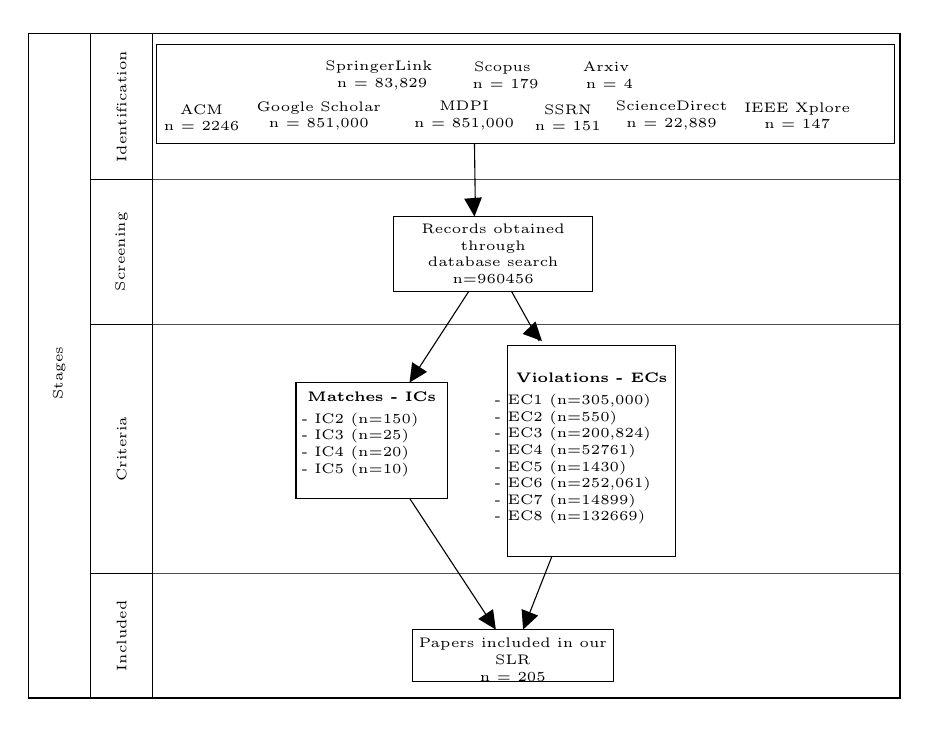
\begin{tikzpicture}[x=0.75pt,y=0.75pt, yscale=-1,xscale=1]
%uncomment if require: \path (0,342); %set diagram left start at 0, and has height of 342

%Shape: Rectangle [id:dp0019014955149456725] 
\draw   (10,10) -- (430,10) -- (430,330) -- (10,330) -- cycle ;

%Shape: Rectangle [id:dp001991157125860177] 
\draw   (10,10) -- (40,10) -- (40,330) -- (10,330) -- cycle ;
%Shape: Rectangle [id:dp904102156184196] 
\draw   (40,10) -- (70,10) -- (70,330) -- (40,330) -- cycle ;
%Shape: Rectangle [id:dp9164832028680756] 
\draw   (40,10) -- (70,10) -- (70,80) -- (40,80) -- cycle ;
%Shape: Rectangle [id:dp844062069727546] 
\draw   (40,80) -- (70,80) -- (70,150) -- (40,150) -- cycle ;
%Shape: Rectangle [id:dp07016298949029287] 
\draw   (40,150) -- (70,150) -- (70,270) -- (40,270) -- cycle ;
%Shape: Rectangle [id:dp5799107359989104] 
\draw   (40,270) -- (70,270) -- (70,330) -- (40,330) -- cycle ;
%Shape: Rectangle [id:dp4056799987768438] 
\draw  [color={rgb, 255:red, 0; green, 0; blue, 0 }  ,draw opacity=0.45 ] (70,10) -- (430,10) -- (430,80) -- (70,80) -- cycle ;
%Shape: Rectangle [id:dp6386898601196207] 
\draw  [color={rgb, 255:red, 0; green, 0; blue, 0 }  ,draw opacity=0.45 ] (70,80) -- (430,80) -- (430,150) -- (70,150) -- cycle ;
%Shape: Rectangle [id:dp2906994943624406] 
\draw  [color={rgb, 255:red, 0; green, 0; blue, 0 }  ,draw opacity=0.45 ] (70,150) -- (430,150) -- (430,270) -- (70,270) -- cycle ;
%Shape: Rectangle [id:dp23551377863706668] 
\draw  [color={rgb, 255:red, 0; green, 0; blue, 0 }  ,draw opacity=0.45 ] (70,270) -- (430,270) -- (430,330) -- (70,330) -- cycle ;

% Text Node
\draw    (72,15) -- (427.5,15) -- (427.5,63) -- (72,63) -- cycle  ;
\draw (93.5,50.5) node  [font=\tiny] [align=left] {\begin{minipage}[lt]{50.33pt}\setlength\topsep{0pt}
\begin{center}
ACM \\ n = 2246
 % Google Scholar Scopus SSRN ScienceDirect MDPI IEEE Xplore SpringerLink 
\end{center}

 \end{minipage}};
% Text Node
% \draw    (121,37) -- (185,37) -- (185,62) -- (121,62) -- cycle  ;
\draw (150,49.5) node  [font=\tiny] [align=left] {\begin{minipage}[lt]{50.24pt}\setlength\topsep{0pt}
\begin{center}
Google Scholar\\n = 851,000
\end{center}

 \end{minipage}};

\draw (220,49.5) node  [font=\tiny] [align=left] {\begin{minipage}[lt]{50.24pt}\setlength\topsep{0pt}
\begin{center}
MDPI\\n = 851,000
\end{center}

 \end{minipage}};
 
% Text Node
\draw (270,50.5) node  [font=\tiny] [align=left] {\begin{minipage}[lt]{50.59pt}\setlength\topsep{0pt}
\begin{center}
SSRN\\n = 151 
\end{center}

\end{minipage}};
% Text Node
\draw (320,49.5) node  [font=\tiny] [align=left] {\begin{minipage}[lt]{50.12pt}\setlength\topsep{0pt}
\begin{center}
ScienceDirect \\n = 22,889
\end{center}

\end{minipage}};
% Text Node
\draw (380.5,49.5) node  [font=\tiny] [align=left] {\begin{minipage}[lt]{50.26pt}\setlength\topsep{0pt}
\begin{center}
IEEE Xplore \ \\n = 147
\end{center}

\end{minipage}};
% Text Node
\draw (180.5,30) node  [font=\tiny] [align=left] {\begin{minipage}[lt]{50.88pt}\setlength\topsep{0pt}
\begin{center}
SpringerLink \ \ \\n = 83,829
\end{center}

\end{minipage}};

% Text Node
\draw (240,30) node  [font=\tiny] [align=left] {\begin{minipage}[lt]{50.88pt}\setlength\topsep{0pt}
\begin{center}
Scopus \ \ \\n = 179
\end{center}

\end{minipage}};

% Text Node
\draw (290,30) node  [font=\tiny] [align=left] {\begin{minipage}[lt]{50.88pt}\setlength\topsep{0pt}
\begin{center}
Arxiv \ \ \\n = 4
\end{center}

\end{minipage}};




% Text Node
\draw    (186,98) -- (282,98) -- (282,134) -- (186,134) -- cycle  ;
\draw (234,116) node  [font=\tiny] [align=left] {\begin{minipage}[lt]{62.52pt}\setlength\topsep{0pt}
\begin{center}
Records obtained through \\database search \\n=960456
\end{center}

\end{minipage}};

%\draw    (186,98) -- (282,98) -- (282,134) -- (186,134) -- cycle  ;
%\draw (400,116) node  [font=\tiny] [align=left] {\begin{minipage}[lt]{62.52pt}\setlength\topsep{0pt}
%\begin{center}
%Records obtained through \\database search \\n=960456
%\end{center}

%\end{minipage}};
% Text Node
\draw (25,173.5) node  [font=\tiny,rotate=-270] [align=left] {\begin{minipage}[lt]{50.39pt}\setlength\topsep{0pt}
\begin{center}
Stages
\end{center}

\end{minipage}};
% Text Node
\draw (55,45) node  [font=\tiny,rotate=-270] [align=left] {\begin{minipage}[lt]{50.31pt}\setlength\topsep{0pt}
\begin{center}
Identification
\end{center}

\end{minipage}};
% Text Node
\draw (55,115) node  [font=\tiny,rotate=-270] [align=left] {\begin{minipage}[lt]{50.24pt}\setlength\topsep{0pt}
\begin{center}
Screening
\end{center}

\end{minipage}};
% Text Node
\draw (55,210) node  [font=\tiny,rotate=-270] [align=left] {\begin{minipage}[lt]{50.12pt}\setlength\topsep{0pt}
\begin{center}
Criteria
\end{center}

\end{minipage}};
% Text Node
\draw (55,300) node  [font=\tiny,rotate=-270] [align=left] {\begin{minipage}[lt]{50.1pt}\setlength\topsep{0pt}
\begin{center}
Included
\end{center}

\end{minipage}};
% Text Node
\draw    (139,178) -- (212,178) -- (212,234) -- (139,234) -- cycle  ;
\draw (175.5,206) node  [font=\tiny] [align=left] {\begin{minipage}[lt]{50.71pt}\setlength\topsep{0pt}
\begin{center}
\textbf{Matches - ICs} 
\end{center}
- IC2 (n=150)\\
- IC3 (n=25)\\
- IC4 (n=20)\\
- IC5 (n=10) \\
% - IC3 (n=\hl{15})\\
% - IC4 (n=\hl{14})\\
% - IC5 (n=\hl{5})\\
% - IC6 (n=\hl{19}) \\
\end{minipage}};
% Text Node
\draw    (241,160) -- (322,160) -- (322,262) -- (241,262) -- cycle  ;
\draw (281.5,213) node  [font=\tiny] [align=left] {\begin{minipage}[lt]{70.21pt}\setlength\topsep{0pt}
\begin{center}
\textbf{Violations - ECs}
\end{center}
- EC1 (n=305,000)\\
- EC2 (n=550)\\
- EC3 (n=200,824)\\ % 2062 + 1 secondary study (Caulo et al.)
- EC4 (n=52761)\\
- EC5 (n=1430)\\
- EC6 (n=252,061)\\
- EC7 (n=14899)\\
- EC8 (n=132669)\\
\end{minipage}};
% Text Node
\draw    (195,297) -- (292,297) -- (292,322) -- (195,322) -- cycle  ;
\draw (243.5,311.5) node  [font=\tiny] [align=left] {\begin{minipage}[lt]{80.33pt}\setlength\topsep{0pt}
\begin{center}
Papers included in our SLR\\n = 205
\end{center}

\end{minipage}};
% Connection
%\draw    (112,59.12) -- (192.67,96.73) ;
%\draw [shift={(195.39,98)}, rotate = 204.99] [fill={rgb, 255:red, 0; green, 0; blue, 0 }  ][line width=0.08]  [draw opacity=0] (8.93,-4.29) -- (0,0) -- (8.93,4.29) -- cycle    ;
% Connection
%\draw    (168.23,62) -- (209.76,96.1) ;
%\draw [shift={(212.08,98)}, rotate = 219.39] [fill={rgb, 255:red, 0; green, 0; blue, 0 }  ][line width=0.08]  [draw opacity=0] (8.93,-4.29) -- (0,0) -- (8.93,4.29) -- cycle    ;
% Connection
\draw    (225,63) -- (225.44,95.23) ;
\draw [shift={(225,98)}, rotate = 265.6] [fill={rgb, 255:red, 0; green, 0; blue, 0 }  ][line width=0.1]  [draw opacity=0] (8.93,-4.29) -- (0,0) -- (8.93,4.29) -- cycle    ;
% Connection
%\draw    (258.36,62) -- (243.35,95.27) ;
%\draw [shift={(242.12,98)}, rotate = 294.28] [fill={rgb, 255:red, 0; green, 0; blue, 0 }  ][line width=0.08]  [draw opacity=0] (8.93,-4.29) -- (0,0) -- (8.93,4.29) -- cycle    ;
% Connection
%\draw    (310.74,62) -- (262.03,96.27) ;
%\draw [shift={(259.58,98)}, rotate = 324.87] [fill={rgb, 255:red, 0; green, 0; blue, 0 }  ][line width=0.08]  [draw opacity=0] (8.93,-4.29) -- (0,0) -- (8.93,4.29) -- cycle    ;
% Connection
%\draw    (358,61.57) -- (277.75,96.79) ;
%\draw [shift={(275.01,98)}, rotate = 336.3] [fill={rgb, 255:red, 0; green, 0; blue, 0 }  ][line width=0.08]  [draw opacity=0] (8.93,-4.29) -- (0,0) -- (8.93,4.29) -- cycle    ;
% Connection
\draw    (222.3,134) -- (195.33,175.48) ;
\draw [shift={(193.7,178)}, rotate = 303.02] [fill={rgb, 255:red, 0; green, 0; blue, 0 }  ][line width=0.08]  [draw opacity=0] (8.93,-4.29) -- (0,0) -- (8.93,4.29) -- cycle    ;
% Connection
\draw    (242.81,134) -- (256.19,158) ;
\draw [shift={(257.51,158)}, rotate = 225.91] [fill={rgb, 255:red, 0; green, 0; blue, 0 }  ][line width=0.08]  [draw opacity=0] (8.93,-4.29) -- (0,0) -- (8.93,4.29) -- cycle    ;
% Connection
\draw    (193.9,234) -- (233.64,294.49) ;
\draw [shift={(235.29,297)}, rotate = 236.69] [fill={rgb, 255:red, 0; green, 0; blue, 0 }  ][line width=0.08]  [draw opacity=0] (8.93,-4.29) -- (0,0) -- (8.93,4.29) -- cycle    ;
% Connection
\draw    (262.2,262) -- (249.52,294.21) ;
\draw [shift={(248.42,297)}, rotate = 291.49] [fill={rgb, 255:red, 0; green, 0; blue, 0 }  ][line width=0.08]  [draw opacity=0] (8.93,-4.29) -- (0,0) -- (8.93,4.29) -- cycle;

\end{tikzpicture}

    \caption{Prisma Flow Chart Diagram}
    \label{F:prismaFlowDiagram}
\end{figure}

\begin{table}
\caption{Papers' Ranking}
\label{T:qualityLevels}
    \begin{tabularx}{\columnwidth}{X l r r}
    \toprule
    Quality Level & Score Range & Count & Percentage \\
    \midrule
    Poor & [0-1.5] & 20 & 9\% \\
    Good & [2-4] & 100 & 49\% \\
    % \st{43}
    Excellent & [4.5-5] & 85 & 42\% \\
    
    \midrule
    Total & --- & 205 & 100\% \\
    % 58
    \bottomrule
    \end{tabularx}
\end{table}

We note that the vast majority of the papers we included in our final reading log ($\sim91\%$) were of good or excellent quality. Hence, we can infer that the data on which we based our SLR are scientifically sound. We also note that the hypen "-" in ~\Cref{tab:paperselection} indicates that they also satisfy that particular research question as well as the other one. For example, in Google Scholar, we note that 85 and 1 paper exclusively address RQ1 and RQ2 respectively, these papers collectively address RQ3 together. ~\Cref{F:prismaFlowDiagram} for Prisma template was obtained from \cite{succi2022}

\section{Results} \label{S:results}

This section summarises the results obtained from reading and extracting the data from the papers we included in the final reading log.

\subsection{Preliminary Clustering} \label{S:preliminaryClustering}

As noted above, we performed this SLR on some of the most popular and trusted databases available to researchers.

We note that we attributed papers to single databases (even if some papers could be found across different databases), based on the chronological order of the searches performed. We also notice that two databases (Google Scholar and IEEE Explore) indexed the most (41 + 41\% $\sim$ 82\%) of the papers included in our reading log. Searches performed on MDPI and ACM rendered the least ($\sim$ 1.9\% each) number of relevant papers amounting to only of the total papers included in the log, while Arxiv accumulated zero number of papers.

\begin{figure}
   \resizebox{\columnwidth}{!}{
    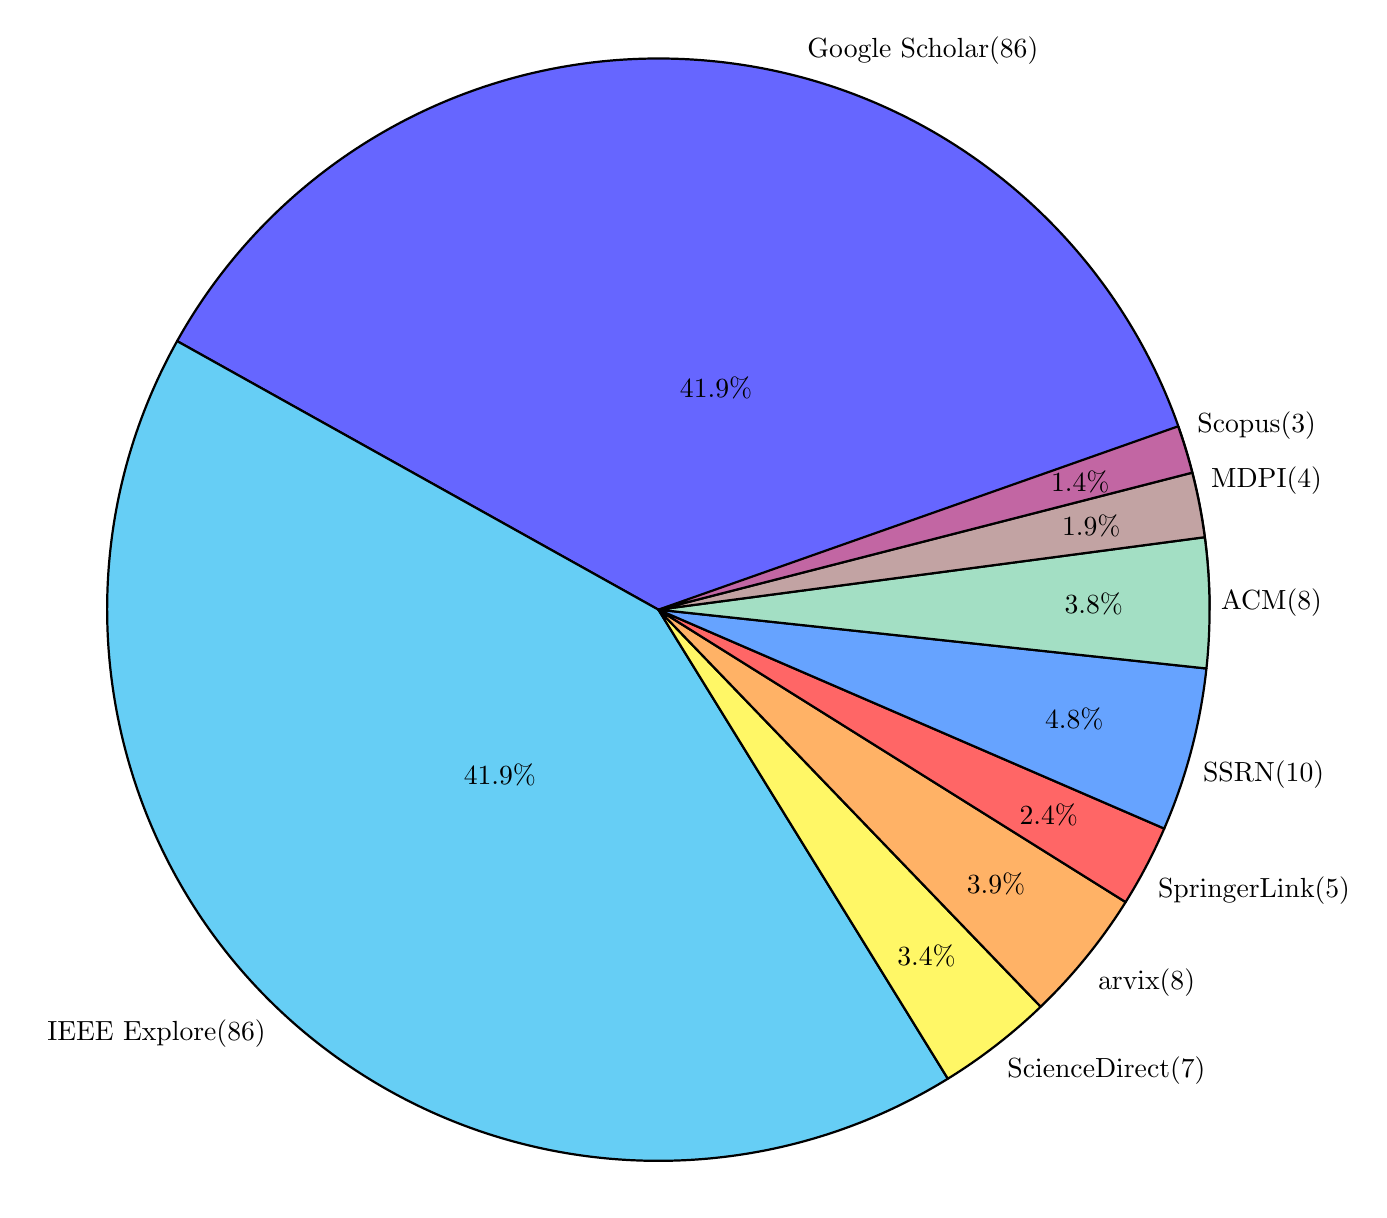
\begin{tikzpicture}
    % We will draw the pie chart here
    
    \pie[radius = 7] {
    41.9/Google Scholar(86),
    41.9/IEEE Explore(86),
    3.4/ScienceDirect(7),
    3.9/arvix(8),
    2.4/SpringerLink(5),
    4.8/SSRN(10),
    3.8/ACM(8),
    1.9/MDPI(4),
    1.4/Scopus(3)}
\end{tikzpicture}
    }
    \caption{Distribution of studies by Database based on search queries}
    \label{F:databasedistribution}
\end{figure}

% This is to address, the fact, that we could have duplicates
Thus, in~\Cref{F:databasedistribution} above and~\Cref{tab:paperselection} above, we only represented papers, which we attributed to a single repository. The attribution was subjective in character and yet followed the following rule. The paper was attributed to one database (e.g. Google Scholar) rather than to the other (e.g., Scopus) based on the chronological order of the searches we performed. We think that while this is perhaps not an ideal practice, it does not constitute a significant problem for this work. 

%Also, presented below, is a distribution of publications , 
\begin{table}
\caption{Database Advantage and Limitations}
\label{T:databaseadvantageandlimitations}
\begin{tabular}{ l  p{3.4cm}  p{3.4cm} }
        \toprule
\textbf{Database}      
& \textbf{Advantages}   
& \textbf{Limitations}   \\
\midrule
Google Scholar & This database is helpful in finding open access articles. It provides papers’ citations data, which is a useful indicator of an article’s popularity within a given scientific community. & Some papers (those not peer-reviewed) can be problematic, a few more are behind a paywall  \\
% \st{43}
Scopus,ScienceDirect and SSRN & Scientific databases with effective and precise search tools and analytic statistics &  Most of its journals as well as search features are behind paywall  \\
 IEEE Xplore & Published papers are all peer-reviewed by leading experts in the field & Paywall  \\
 SpringerLink & High Quality peer-reviewed papers, with reasonably priced access & Paywall  \\
 MDPI & Peer-Reivewed and fast reviewd & Not as reputable as other journals \\

\bottomrule
\end{tabular}
\end{table}

We also present  the geographical distribution of the studies we included in our log (based on first author's affiliation).~\Cref{F:countrydistribution} shows that the studies we selected have been published in at least 13 countries. The Other represents countries with publications less than or equal to 3, which includes Japan, Bangladesh, Greece, etc. This ensures a sufficient degree of cultural diversity for our reading log. 
 \begin{figure}
    \resizebox{\columnwidth}{!}{
    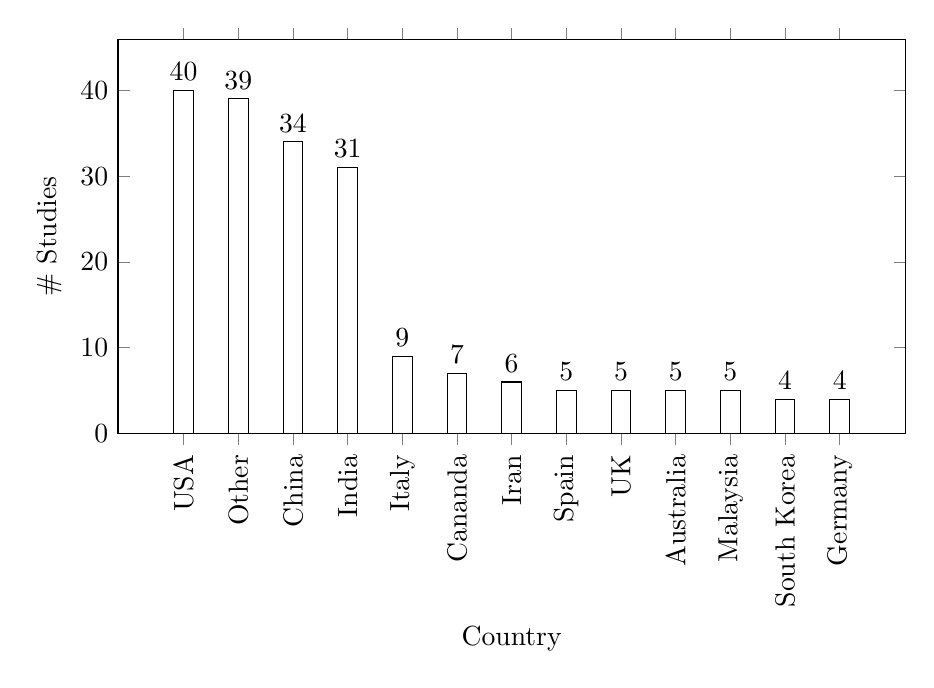
\begin{tikzpicture}
  \centering
  \begin{axis}[
%   small,
        scale only axis,
        ybar,
        % axis on top,
        height=\axisHeight,
        width=\axisWidth,
        bar width=\barWidth,
        % x=-0.5,
        % ymajorgrids,
        % tick align=inside,
        % major grid style={draw=white},
        enlarge y limits={value=.02,upper},
        % legend pos = north east,
        % legend style={at={(1, 1.2)},anchor=north},
        ymin=0, ymax=45,
        % axis x line*=bottom,
        % axis y line*=right,
        % y axis line style={opacity=0},
        % tickwidth=0pt,
        % enlarge x limits=true,
        % legend style={
        %     at={(0.3,0.95)},
        %     anchor=north,
        %     legend columns=-1,
        %     /tikz/every even column/.append style={column sep=0.5cm}
        % },
        ylabel={\# Studies},
        xticklabel style={rotate=90},
        symbolic x coords={
USA, 
Other,
China,
India,
Italy,
Cananda,
% (Iran, 1)
% (Italy, 1)
Iran,
Spain,
% (Norway, 1)
UK,
Australia,
Malaysia,
South Korea,
Germany,
% USA,
% India,
% China,
% Finland,
% Brazil,
% Canada,
% England,
% Germany,
% Australia,
% Belgium,
% Iran,
% Italy,
% Japan,
% Malaysia,
% Norway,
% Spain,
% Sweden,
% Taiwan
},
        xlabel = {Country},
       xtick=data,
       nodes near coords={
        \pgfmathprintnumber[precision=0]{\pgfplotspointmeta}
       }
    ]
   \addplot [draw=barDrawColor,fill=barFillColor] coordinates {
 % (India, 12)
(USA, 40)
(Other, 39)
(China, 34)
(India, 31)
(Italy, 9)
(Cananda, 7)
% (Iran, 1)
% (Italy, 1)
(Iran, 6)
(Spain, 5)
% (Norway, 1)
(UK, 5)
(Australia, 5)
(Malaysia, 5)
(South Korea, 4)
(Germany, 4)
};

    % \legend{Publication Country}
  \end{axis}
  \end{tikzpicture}
    }
     \caption{Distribution of studies by country of origin, based on first author's affiliation}
    \label{F:countrydistribution}
 \end{figure}

 \begin{figure}
    \resizebox{\columnwidth}{!}{
     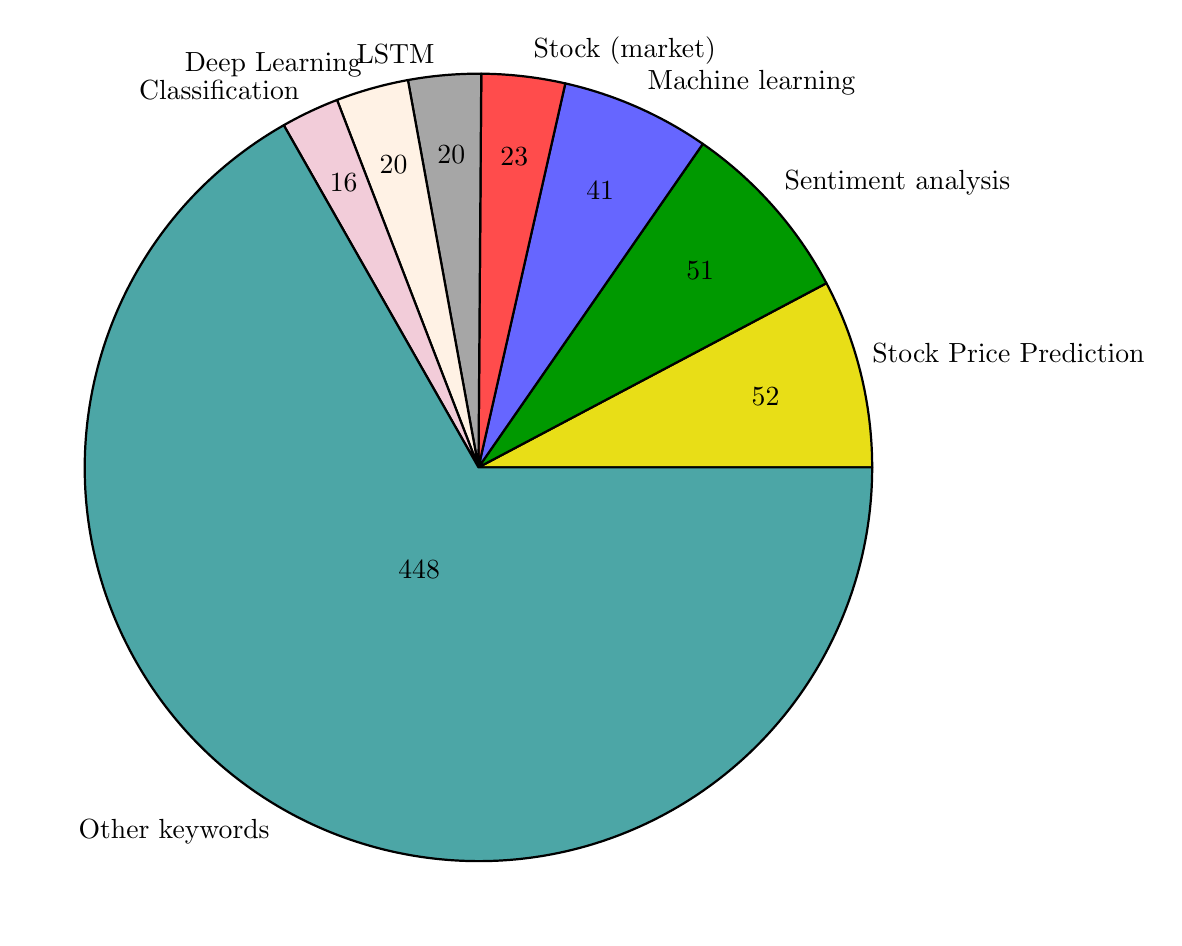
\begin{tikzpicture}
 
\pie[
    color = {
        yellow!90!black,
        green!60!black,
        blue!60,
        red!70, 
        gray!70,
        orange!10,
        purple!20,
        teal!70
        }, 
    sum = auto,radius=5
]{52/Stock Price Prediction,
    51/Sentiment analysis,
    41/Machine learning,
    23/Stock (market),
    20/LSTM,
    20/Deep Learning,
    16/Classification,
    448/Other keywords}
 
\end{tikzpicture}
     }
     \caption{Distribution of keywords}
     \label{F:keywords}
 \end{figure}


We also display a distribution of publications by year from 1996-2022 ~\Cref{F:publicationbyyear}. We can clearly see a rise in use of machine learning methods in asset allocation/forecasting, including the use of NLP techniques. We have also presented the same data in,~\Cref{T:paperdistributionbyfiveyear} where for simplicity the distribution is shown over a period of 5-years.


 \begin{figure}
    \resizebox{\columnwidth}{!}{
     %\begin{tikzpicture}
%\centering
%\begin{axis} [ 
 %   %tiny,
  %  scale only axis,
  % ybar, 
   % xmin=1996, xmax=2022,
   % ymin=0, ymax=45, 
   % bar width=.60*\barWidth,
   %grid=false,
   % height= \axisHeight,
   %width= \axisWidth, 
   %enlargelimits=false,
    %axis equal image,
	%x tick label style={/pgf/number format/1000 sep=},
%	xlabel=Publication Year,
%%	ylabel=\# Studies,
  %  xticklabel style={rotate=90},
    %%% FROM HERE UPWARDS ITS ORIGINAL %%%
	%xtick={
 %%% BORROWED FROM COUNTRY %%%
 \begin{tikzpicture}
  \centering
  \begin{axis}[
        tiny,
        scale only axis,
        ybar,
        % axis on top,
        height=\axisHeight,
        width=\axisWidth,
        bar width= 0.60*\barWidth,
        % x=-0.5,
        % ymajorgrids,
        % tick align=inside,
        % major grid style={draw=white},
        enlarge y limits=false,
        %axis equal image,
        x tick label style={/pgf/number format/1000 sep=},
        % legend pos = north east,
        % legend style={at={(1, 1.2)},anchor=north},
        xmin=1996, xmax=2022,
        ymin=0, ymax=45,
        % axis x line*=bottom,
        % axis y line*=right,
        % y axis line style={opacity=0},
        % tickwidth=0pt,
        % enlarge x limits=true,
        % legend style={
        %     at={(0.3,0.95)},
        %     anchor=north,
        %     legend columns=-1,
        %     /tikz/every even column/.append style={column sep=0.5cm}
        % },
        %ylabel={\# Studies},
        xlabel=Publication Year,
	    ylabel=\# Studies,
        xticklabel style={rotate=90},
        symbolic x coords={
1996,
1998,
2001,
2002,
2004,
2005,
2007,
2008,
2009,
2010,
2011,
2012,
2013,
2014,
2015,
2016,
2017,
2018,
2019,
2020,
2021,
2022,
}, 
    %ytick={5,10,15,20,25,30,35,40,45,50},
    % enlarge x limits=true,
% 	enlargelimits=0.05,
% 	legend style={at={(0.5,-0.1)},
% 	anchor=north,legend columns=-1},
% 	ybar interval=0.7,
     % nodes near coords={
      % \pgfmathprintnumber[precision=1]{\pgfplotspointmeta}
      %}
]
\addplot [draw=barDrawColor,fill=barFillColor] coordinates {
    (1996, 1)
    (1998, 1)
    (2001, 1)
    (2002, 1)
    (2004, 1)
    (2005, 1)
    (2007, 2)
    (2008, 1)
    (2009, 5)
    (2010, 2)
    (2011, 3)
    (2012, 4)
    (2013, 3)
    (2014, 1)
    (2015, 7)
    (2016, 7)
    (2017, 11)
    (2018, 13)
    (2019, 24)
    (2020, 35)
    (2021, 37) %     (2013, 5)
    (2022, 43) %    (2020, 5)
    % (2021, 0)
};
\end{axis}
\end{tikzpicture}

     }
     \caption{Distribution Of Studies By Year}
     \label{F:publicationbyyear}
 \end{figure}


\begin{table}
\caption{Paper Distribution Around 5-year Period}
\label{T:paperdistributionbyfiveyear}
\begin{tabularx}{\columnwidth}{X r r}
\toprule
Year Range  & Count & Percentage \\
\midrule
1996-2004  & 4 & 1.9\% \\
2005-2010  & 11 & 5.2\% \\
% \st{43}
2010-2015 & 20 & 9.6\% \\
2016-2020 & 90 & 43.2\%\\
2021-2022 & 80 & 38.4\%\\


\midrule
%Total & --- & 53 & 100\% \\
% 58
%\bottomrule
\end{tabularx}
\end{table}

We also, visually display the distribution of Journals that contained collected papers in~\Cref{F:journalsdist}. Others include journals such as Journal of Econometrics, Hindawi, Financial Letters etc. All of which are $\le 3$.

\begin{figure}
   \resizebox{\columnwidth}{!}{
    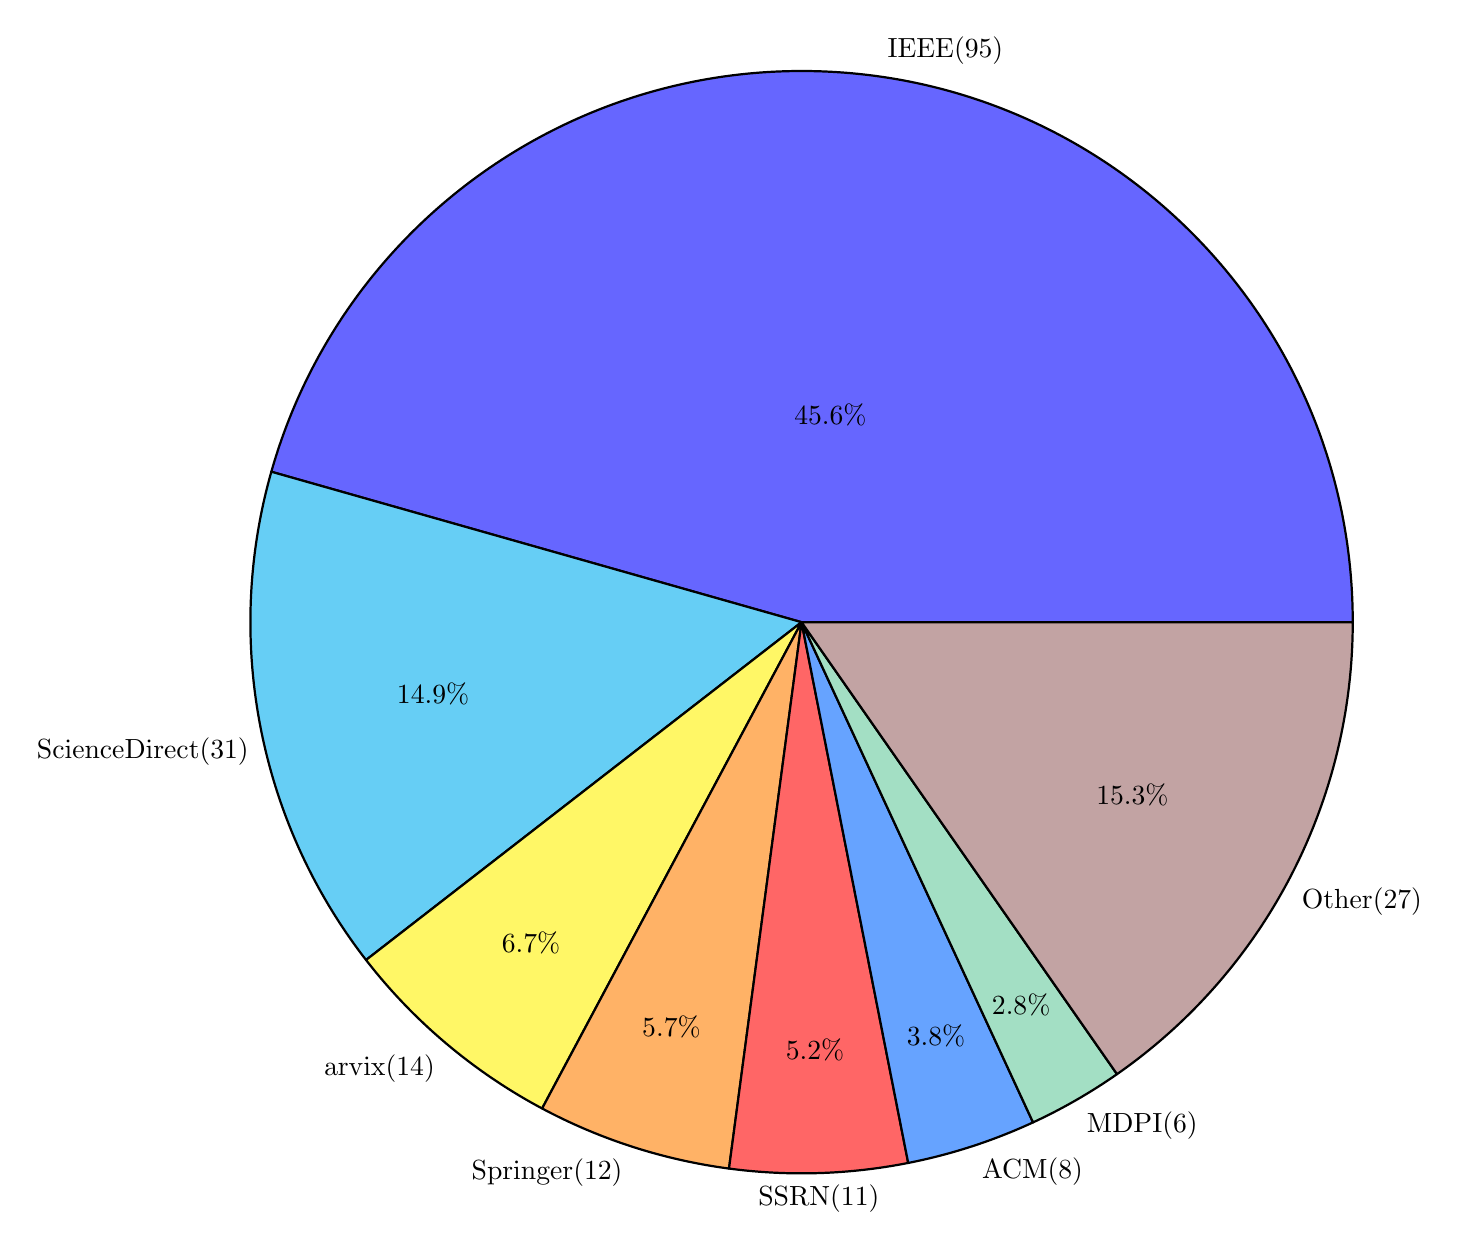
\begin{tikzpicture}
    % We will draw the pie chart here
    
    \pie[radius = 7] {
    45.6/IEEE(95),
    14.9/ScienceDirect(31),
    6.7/arvix(14),
    5.7/Springer(12),
    5.2/SSRN(11),
    3.8/ACM(8),
    2.8/MDPI(6),
    15.3/Other(27)}
\end{tikzpicture}
    }
    \caption{Distribution of studies By Journals}
    \label{F:journalsdist}
\end{figure}

\subsection{Further Clustering}
We present further clustering based on the following parameters a) Algorthims, b) Datasets, and c) Metrics.

In addition, we also clustered the datasets used in the papers included in the final reading log. It is worth noting that a single dataset was found in multiple articles and use of certain algorithms were prevalent in many articles.~\Cref{T:algorithms} lists the algorithms used for training models and the statistics of their usage. We observed that LSTMs and SVMs were the most frequently mentioned algorithms. We concluded that it can probably be considered as the most widely used in the field.


\begin{table}
\caption{Algorithms Used}
\label{T:algorithms}
\begin{tabularx}{\columnwidth}{X r r}
\toprule
Algorithm  & Count & Percentage \\
\midrule
SVM  & 43 & 20\% \\
LSTM  & 43 & 20\% \\
% \st{43}
Naive Bayes & 22 & 10.5\% \\
ARIMA & 17 & 8\%\\
Random Forest & 12 & 5.7\% \\
ANN & 11 & 5.2\%\\
Linear Regression & 11 & 5.2\% \\
kNN & 10 & 4.8\%\\
Logistic Regression & 9 & 4.3\% \\
RNN & 7 & 3.3\% \\
CNN & 6 & 2.8\% \\
Decision Trees & 6 & 2.8\% \\
GRU & 6 & 2.8\% \\
GAN & 3 & 1.4\% \\
Others & 102 & 49\% \\


\midrule
%Total & --- & 53 & 100\% \\
% 58
%\bottomrule
\end{tabularx}
\end{table}


"Other" Algorthims mentioned in~\Cref{T:algorithms} include k-Means Clustering, Transformer architectures, P-Trees, XGBoost etc. All of these algorithms used were less $\le 2$ in number. We also note a discrepancy in the number of algorithms used compared to total number of papers. This is due to the fact that some algorithms appeared in more than one papers, or used 2 or more algorithms in a pipeline as their solution. 

Furthermore,~\Cref{T:metrics} below displays a list of metrics used for evaluating a model.

\begin{table}
\caption{Metrics Used}
\label{T:metrics}
\begin{tabularx}{\columnwidth}{X r r}
\toprule
Metrics & Count & Percentage \\
\midrule
Accuracy & 60 & 28.8\% \\
R-Squared  & 39 & 18.75\% \\
% \st{43}
RMSE & 32 & 15.3\% \\
MSE & 15 & 7.2\%\\
MAE & 15 & 7.2\% \\
Precision & 15 & 7.2\%\\
Recall & 14 & 6.7\% \\
MAPE & 10 & 4.8\%\\
F-Score & 8 & 4.3\% \\
ROC-AUC & 4 & 1.9\% \\
MCC & 3 & 1.4\% \\
Correlation & 3 & 1.4\% \\
Sharpe Ratio & 3 & 1.4\% \\
Others & 18 & 8.6\% \\


\midrule
%Total & --- & 53 & 100\% \\
% 58
%\bottomrule
\end{tabularx}
\end{table}

Others here include Average absolute difference rate, Beta Value, Weighted Recall etc. All of these metrics are of count $\le 2$

Finally, we present in~\cref{T:datasetsused}, list of datasets used and also count for each.

\begin{table}
\caption{Datsets Used In Studies}
\label{T:datasetsused}
\begin{tabularx}{\columnwidth}{X r r r}
\toprule
Dataset  & Count & Percentage \\
\midrule
Twitter & 25 & 12\% \\
S\&P  & 21 & 10\% \\
% \st{43}
Yahoo Finance & 12 & 5.7\% \\
NASDAQ & 11 & 5.2\%\\
Reuters Website & 5 & 2.4\% \\
NSE & 5 & 2.4\%\\
NYSE & 5 & 2.4\% \\
Google Trend Index & 4 & 1.9\%\\
Others & 139 & 66.8\% \\

\midrule
%Total & --- & 53 & 100\% \\
% 58
%\bottomrule
\end{tabularx}
\end{table}

The Others included datasets like Nifty, Shanghai Stock Exchange, etc. Others include datasets that are $\le 3$ in total frequency of papers.

\section{Discussion} \label{S:discussion}

\subsection{Datasets Used} \label{S:datasets used}

Twitter, S\&P and Yahoo Finance are the most predominant datasets that are used by the researchers in our SLR as shown in ~\Cref{T:datasetsused}. The reason for this could be due to the fact that these are publicly available datasets, and are are typically huge in terms of number of sample points. 

NASDAQ, Reuters constituted the remaining dominant datasets used by researchers. Twitter was the dominant source for Stock prediction using News articles \citep[see][]{Dong2020,Bollen2011,Sharma2019}.

Some Articles used ML models for predicting sales performance using Blogs like in \cite{Liu2007}. Other articles, collected and built their own custom collection of stocks, but did not mention the source as in \cite{Song2020}

News sites, as well as encyclopedia entries, are commonly used for text classification tasks because they offer a broad set of topics and (or) an abundance of texts.


\subsection{Stock Preprocessing/Text Preprocessing} \label{S:preprocessing}
This section is devoted in commenting the on the preprocessing steps that were used before applying any Machine Learning models. 

In terms of Stock pre-processing, some authors used predictor variables directly from publicly available datasets like S\&P 500 \citep[see][]{Feng2018}, while some drastically change their data representation, converting them into graph structures, that takes correlation of asset returns to build connectivity between assets \citep[see][]{son2022,Uddin2021}, while some converted the stocks into embeddings that are part of graph neural network pipelines \citep[see][]{Wu2019}. As found in \cite{Wu2019}, embeddings of stocks and news articles, returned best performance in terms of Sharpe Ratio and Profit\&Loss. \cite{Shynkevich2015} divided pre-processing into three steps: feature extraction, selection and representation. Author mentioned that the Bag-of-Words approach is used for feature extraction, and all articles are processed in the following way. Following that, words with capital letters are converted to lowercase, words with two or fewer characters are filtered out, and stop words are deleted. Finally, Porter's stemming algorithm is applied to each word in order to extract stems in order to treat different forms of the same word equally.

\subsection{Algorithms} \label{S:algorithms}
As observed from~\Cref{T:algorithms}, SVM is the most popular used algorithm in our collection of studies. SVM works well for linearly separable data, however, if data is non-linear, SVM will employ kernel tricks to project the data into higher dimension , and try to separate the data in that dimension. SVM however, does not perform well with noisy data set, and does not work well with large datasets, that are prevalent in the finance industry. 

Other approaches for forecasting Stock prices, was Random Forest as shown in \cite{sadorsky2021}. A 20-day forecast horizon, tree bagging and random forests methods produce accuracy rates of between 85\% and 90\% while logit models produce accuracy rates of between 55\% and 60\%. Random Forests are highly interpretable, and according to this study, showed more promising results. 

\cite{ENKE2005} was one of the first instance in our collection of using Neural networks(NN), as well as using General Regression Neural Networks(GRNN). They made an importatnt point that eventhough GRNN provides better performance measurement, they did not generate as much profit compared to the vanilla NN. The NN showed better prediction of signs on highly volatile periods, hence paramters should be trained to make robust predicitons where higher returns are available.

The Other most popular algorthim that was used LSTM. The LSTM model was either used as  a standalone architecture \citep[see][]{Koudjonou2020, shen2021}, or it was used with combination of other models like CNN-BiLSTM as in \cite{wang2021stock} and combining traditional Time Series methods like ARIMA with LSTM \citep[see][]{hua2020}

Other methodologies include Reinforcement Learning in stock trading using Deep Q networks \citep[see][]{dang2019}, as well as using and ensemble of Deep Q-learning agents as in \cite{carta2021}. Others used other policy optimization procedures like PPO, A2C as in \cite{Durall2022}

Graph based approaches have also been in the rise, as it is seems natural to consider stocks as nodes of graphs as in \cite{son2022,Fazli2021}

Explainable AI is one of the other factors that should taken into account when building a robust and interpretable Neural Network, as we are allocating clients' resources and financial assets. \cite{Golnoosh2022} uses Shapely values of their complex ML model, can contribute to the shift in Z-score of their portfolio. Shapely Values and LIME were also used in \cite{Jakubowski2022} for asset failure prediction. LIME and Shapely values are quite easy to understand but fail to scale for large feature space. Other researchers opted to integrate fuzzy logic into system as in \cite{chen2014, xie2021}

Further other methodologies applied heuristic based optimization approaches like Genetic Algorthim \citep[see][]{thakkar2022information,CHEN_2020}, fruitfly Optimization \citep[see][]{tian2020}

\cite{Sharma2019} used in his work Generalized additive models (GAM). GAMs combine the concept of additive models with the standard generalized linear models. By estimating nonparametric functions of predictor variables that are connected to the dependent variable via some link function, generalized additive models aim to maximize prediction quality of a dependent variable from many distributions. The GAM model has the advantage of easily decomposing and incorporating new components, such as identifying and incorporating a new source of seasonality.

Algorithms like AdaBoost and Naive Bayes were used in the article \cite{Haider2011}. To correctly identify the weights of the parameters, AdaBoost calls a weak classifier repeatedly in a series of rounds and The Naives Bayes classifier constructs the model using estimator classes. The precision values of numerical estimators are determined by analyzing the training data.

To conclude, there are a number of ways and approaches to time series stock/ asset prediction/forecasting. Nowadays, NN based approaches can be considered a state-of-the-art approach being the one that is most widely used by researchers. The main advantage of NN is that in most of the cases it outperforms other approaches. Its major limitation is that it requires a lot of trials to succeed because none knows exactly, at the time of writing at least, the reason for this superior performance. This means that one needs to try a lot of different combinations of hyperparameters and different preprocessing techniques in order for the model to achieve optimal performance.


\subsection{Quality Assessment Metrics}

 Fortunately, most papers in our SLR, use accuracy in combination with other representative metrics. For example, F-1 Score, Recall and Precision was used with accuracy. F-1 score eliminates the main limitation of accuracy and leads to more precise and reliable results.

 For asset prediction/forecasting, $R^2$ was used. It was used in \cite{Zhang2022, Chen2019, Uddin2020,son2022, Wu2019, Li2020, huang2021} and others. $R^2$ has a lot of issues, R-squared does not measure goodness of fit. It can be arbitrarily low when the model is completely correct, it can be arbitrarily close to 1 even if the model is completely wrong, to name a few. Thankfully, most of the researchers also compared it with other metrics like adjusted $R^2$. 

Another important metric seen in quantitative financial literature, including our study, is Sharpe Ratio. It was used in \cite{son2022} for example. Sharpe ratio is simple formula , but it relies too much on standard deviation and treatment of volatility as the same.

Most popular metrics among stock price time series prediction papers is Mean Squared Error (MSE), Mean Absolute Error (MAE) and Root Mean Square Error (RMSE). For example, all these metrics have been used in these articles: \cite{Dong2020}, \cite{Huan2020}, \cite{Guo2020}, \cite{Yu2019}, \cite{Yu2017} and \cite{Ray2021}.
Mean Squared Error (MSE) and Root Mean Square Error (RMSE) penalize large prediction errors in comparison to Mean Absolute Error (MAE). However, because it uses the same units as the dependent variable, RMSE is more widely used than MSE to compare the performance of the regression model to other random models. In comparison to a non-differentiable function like MAE, MSE is a differentiable function that makes it easier to perform mathematical operations. As a result, despite being more difficult to interpret than MAE, RMSE is often used as the default metric for calculating Loss Function in many models.

Based on the statistical analysis performed above, it seems reasonable and appropriate to summarize the information obtained and to conduct a critical review of our research questions, which is what we will do next.


\section{Critical Review of Research Questions}

\subsection{Analysis of RQ1}\label{S:analysisRQ1}
From The papers collected, there is a strong representation of LSTMs being used for Time Series prediction. But as mentioned in \cite{Feng2018}, LSTMs seem to be overly optimistic and they predict less market crashes. A big problem with LSTMs is that they also require lots more training time, especially on large datasets, and tend to overfit due to their complex and expressive structure.

\cite{Cong2022} applied an interpretable tree based method, called P-Tree to generate a stochastic discount factor model and test assets for cross-sectional asset pricing. Unlike other tree algorithms, P-Trees
accommodate imbalanced panels of asset returns and grow under the no-arbitrage condition. The model is quite simple, requires little training time, and deals with non-linearity, with the added benefit of being highly interpretable. 

\cite{son2022} establishes a graph based approach to asset pricing.To reflect the connectedness between asset returns for risk exposure estimation, they used a graph convolutional network (GCN), which takes into account the graph structure between firms, rather than a simple neural network. They also presented a way to construct a graph of firms that fits our goal, asset pricing, using the correlation of returns. Second, They proposed a forward stagewise modeling architecture that sequentially adds latent factors to inherit factors from the latent factor model of the previous step, such as an observable factor model or PCA-based latent factor model. The model achieved state of the art performance and beats every other benchmark model, the model also achieved the highest Sharpe ratio of the tangency factor portfolio.

\subsection{Analysis of RQ2}\label{S:analysisRQ2}
Most successful and applicable for stock price time series prediction models is LSTM and ARIMA.

Social media content contains a wealth of important information about the stock. The stock financial index variables can only represent the development trend of the stock price, but investor sentiment can describe the potential trend of the stock price, which is usually overlooked in traditional prediction methods. \cite{Huan2020} used deep learning technology to extract text features that can represent investor sentiment and greatly improve prediction performance by using an LSTM-based model.

As found in \cite{Mehta2021}, the ARIMA model performs best when forecasting short-term results, while the LSTM model performs better when forecasting long-term results. Because the user must run the model daily for each stock in the stock market, we need short term prediction to be more accurate. For this scenario, we do not need long term prediction to be more accurate, so the ARIMA model provides the best RMSE score.

The information presented in the collected dataset is in raw form. To remove attribute bias in model development, the data should be cleaned for empty observations and scaled. Each neural network approach employed in \cite{AlAradi2020}, had a unique treatment and selection criterion as in other works.

\subsection{Analysis of RQ3}\label{S:analysisRQ3}

\cite{haq2021} described an accuracy amount of 59.44 for their STOCKNET + MFSS method, outperforming various methods in caparison, like RAND and ARIMA models.

\cite{Li2020} displayed a supreme performance of neural based methods. Showing a result of 2.9($10^-5$) $R^2$ value, in comparison to statistical methods.

\cite{qiu2020} displayed, an RNN based model, returned a MSE of 0.2592, displaying better peroformance. 

 \cite{shen2021} used an LSTM network for effective multinational trade forecasting. It had smaller values of root mean square error (RMSE) and mean absolute percentage error (MAPE) than did time-series models and economic structural models. On the export forecast, RMSE improved by 17.048\%

 As we can see, over the years, even on completely different datasets and data representation, Neural Network models, showed improved performance over the years.

 \subsection{Synoptic Summary}
~\Cref{T:synoptic summary} presents as summary of our results to our research questions tackled in our study.

We identified two main approaches that are used for asset evolution. The first one being, the standard model of using Time Series stocks, and predict their prices in a given window as shown in \cite{dhafer2021}. The other being that they mine text/new articles as displayed in \cite{Gidfalvi2001UsingNA} and \cite{dhafer2021}, which used BP Neural Networks based on public opinion. Typically for the second method, old ML methods like Naive Bayes are being used, or small parameter sized neural network models.

From the methods mentioned in ~\Cref{S:algorithms}, we have identified a few promising approaches. One being mentioned in \cite{sarmah2022}, which uses Learnt embedded Representation of Stock Correlation Matrix. We can further extract textual information uses State of the Art Models like FinBert and further embed such information in our graph structure. 
 
 \begin{table}
\caption{Synoptic summary Of Our Results}
\label{T:synoptic summary}
\begin{tabularx}{\columnwidth}{X p{6.0cm}}
\toprule
RQs & Summary \\
\midrule
RQ1 & A lot of methods are used in asset pricing/forecasting. The most dominant model is LSTM, followed by SVM, Random Forest, GRU, and other NN based approahces like attention Graph Neural Networks \\
RQ2  &  Most popular models for time series stock price forecasting is Long short-term memory (LSTM) and Autoregressive integrated moving average (ARIMA). The ARIMA model performs best when forecasting short-term results, while the LSTM model performs better when forecasting long-term results. \\
% \st{43}
RQ3 & Researchers used a list of metrics, with $R^2$ and MSE being the most common for most regression/time series prediction tasks, and Accuracy being the most coming for classification  \\


\midrule
%Total & --- & 53 & 100\% \\
% 58
%\bottomrule
\end{tabularx}
\end{table}

\section{Limitations, Threats to Validity and Review Assessment}\label{S:limitationsThreatsAssessment}

The analysis of the potential weaknesses of a research work plays a fundamental role in encouraging readers to think more deeply about the topic  as well as in appreciating possible future research directions. In this section, we thus adopt a critical stance on our findings. More specifically, we reflect on a few issues that may have influenced the objectivity, transparency, reproducibility, and academic soundness of our research.  

\subsection{Limitations}\label{S:limitations}
We start by analyzing circumstances and conditions that may limit the relevance and significance of our work. In this context, we might consider two aspects as potentially detrimental to our research:

First, one may see as problematic the fact that we searched only six databases. However, we note that the databases we searched are the most frequently used by researchers in computer science. In addition, one of such databases (Google Scholar) aggregates most of the contents available on other indexes. Thus, it is safe to assume that despite being run on a limited number of databases, our searches were quite comprehensive (more on this in~\cref{S:threats} below)
    % \item The second potential limitation on our work is that we 
Second, one may object that one of our inclusion criteria (English requirement) limited our research capability. Cross-cultural issues have become especially important in modern science . We are aware of these issues and recognize them as vitally important for a fair characterisation of scientific findings. However, given that most publications on the topic are written in English, and since leading journals in the field only accept submission in this language, we believe the restriction we adopted is neither unusual nor unjustified. In any case, the geographical distribution of our studies (Figure 3) demonstrates that there is sufficient cultural variability among the studies we included in our reading log.

\subsection{Threats to Validity}\label{S:threats}

Next, we address a series of possible biases that could cast doubt on the legitimacy or general validity of our work.. These are:
\begin{paraenum}
\item retrieval bias,
\item selector bias,
\item expectation bias, and
\item within-study bias..
\end{paraenum}

\textbf{Retrieval bias:} may occur when the articles selected for inclusion are inadequate or when the searches performed by the authors are partial or incomplete. To avoid this bias, we conducted comprehensive searches on several different databases (six) and did not put any restriction on year of publication. In addition, we only selected high-quality articles, as shown in subsection analysis above in~\cref{S:qualityAssessment} and obviously included only works that matched our research topic.

\textbf{Selector bias:} occurs when the studies selected for inclusion in the reading log are affected by the authors' previous knowledge of the topic. In brief, when the findings are collected subjectively. To avoid the occurrence of this bias, we performed all the searches collaboratively. In other words, each member of the team was directly involved in them. In addition, to safeguard objectivity, team members were also asked to cross-check the activities of other members. 

\textbf{Expectation bias:} can be considered as an extension of the \emph{Selector bias} and typically occurs when data extraction and synthesis is severely constrained by the authors' conscious or unconscious expectations about the results. Our research team consists of academics, students, and industry practitioners. Furthermore, it comprises specialists in machine learning, engineers, and AI scientists, thus it draws from various backgrounds and relies on multiple scientific approaches. Given the multidisciplinary character of our research team and its interdisciplinary stance, we believe we managed to reduce the occurrence of this bias to the minimum.

\textbf{Within-study bias:} develops as a result of a deficiency of data extraction templates. For this purpose, we designed a data extraction template (on Google sheet) and each team member actively participated in filling it.


\section{Conclusion}\label{S:conclusion}
The aim of this Systematic Literature Review was to investigate the usage of Machine Learning in Asset Evolution/Forecasting. This study attempted to answer the following research questions \textbf{RQ1}: What are the most effective ML models to predict evolution of an asset in the financial market? \textbf{RQ2}: What the existing approaches for forecasting stock price trend based on news/tweets or textual data? and \textbf{RQ3}: How accurately can machine learning models predict the stock price?

With regards to \textbf{RQ1}, we found a high representation of studies using LSTMs either as base models or standalone models, and showed to be highly effective. Concerning \textbf{RQ2}, we found LSTM and SVMs dominate the modelling part, which is usually preceded by embeddings. With respect to \textbf{RQ3}, we can state that effectiveness in identification is dependent on the data and on the algorithms used. \cite{shen2021} showed a RMSE improvement of 17.048\%, \cite{qiu2020} returned an MSE of 0.2592.

Our results may also suggest that stock price prediction could be heavily improved using textual data and the appropriate embeddings. In any case, further work is to corroborate any of these speculations.
We nevertheless hope that this systematic literature review will broaden interest in using hybrid sources for financial asset evolution using Machine Learning and will provide new grounds for more detailed explorations into these extraordinarily rich and fascinating set of phenomena.

% Bibliography
\nocite{*}
\begin{doublespacing}
\bibliographystyle{rfs}
%\bibliographystyle{plainnat}
\bibliography{RHSbib}
\end{doublespacing}

\clearpage

% Print end notes
%\renewcommand{\enotesize}{\normalsize}
%\begin{doublespacing}
%  \theendnotes
%\end{doublespacing}

% Figures and tables, showing how to structure captions
\clearpage

% \ 
% \vfill
% \begin{figure}[!htb]
% \centerline{\includegraphics[width=7in]{Figure1}}
% \noindent\caption{}
% {\bf Structure of model: capital can be invested in a bank sector and an equity sector.} 

% An intermediary has the expertise to reallocate capital between the sectors and to monitor bank capital against bank crashes. \label{fig:0}
% \end{figure}
% \vfill
% \ 
\end{document}
